\section{Theorie}
\label{sec:Theorie}


\subsection{Allgemeines}
Brückenschaltungen liefern eine sehr genaue Messung von komplexen und
realen Widerständen. Durch Parallelschalten von Widerständen entsteht eine
messbare Brückenspannung, über welche man einen unbekannten Widerstand
berechnen kann.
Bei der sogenannten abgeglichenen Brückenschaltung werden variable
Widerstände eingesetzt, die so verändert werden, dass die Brückenspannung
verschwindet.
Dann kann über die Kirchhoffschen Gesetze, also die Maschenregel

\begin{equation}
  \sum_k U_k = 0,
\end{equation}

die besagt, dass die Summe der Spannungen in einer Masche Null ist,
und die Knotenregel

\begin{equation}
  \sum_k I_k = 0,
\end{equation}

die besagt, dass die Summe der Ströme in einem Knoten null ist, der unbekannte
Widerstand bestimmt werden.
Den grundlegenden Aufbau einer solchen Schaltung ist in Abbildung
\ref{fig:AllgBr} dargestellt.

\begin{figure}[h]
  \centering
  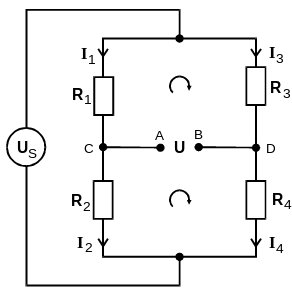
\includegraphics[height=6.25cm]{AllgBr.png}
  \caption{Allgemeiner Aufbau einer Brückenschaltung \cite{anleitung}}
  \label{fig:AllgBr}
\end{figure}

Die Brückenspannung wird zwischen den Punkten $A$ und $B$ gemessen und die
Justierung findet an den variablen Widerständen $R_3$ und $R_4$ statt.
Für die Brückenspannung $U_B$ gilt dann im Allgemeinen

\begin{equation}
  U_B = \frac{R_2R_3 - R_1R_4}{(R_3+R_4)(R_1+R_2)} \cdot U_S
  \label{eqn:Brs}
\end{equation}

mit der Speisespannung $U_S$.
Im Falle einer abgeglichenen Brückenschaltung, ist $U_B = 0$, also
ist in diesem Fall

\begin{equation}
  R_1 = R_2\frac{R_3}{R_4}.
  \label{eqn:AllgBrW}
\end{equation}


\subsection{Wheatstonesche Brücke}

Bei der Wheatstoneschen Widerstandsmessbrücke, die in Abbildung
\ref{fig:WheBr} abgebildet ist, wird für die
Widerstände $R_3$ und $R_4$ ein Potentiometer eingesetzt.
Bei diesem Gerät wird zwischen
drei Knoten ein Gesamtwiderstand angelegt, der dann zwischen dem ersten und
zweiten und dem zweiten und dritten Knoten varriiert, aber in Summe konstant
ist. Als Nullindikator kann zum Beispiel ein Oszilloskop verwendet werden.

\begin{figure}[h]
  \centering
  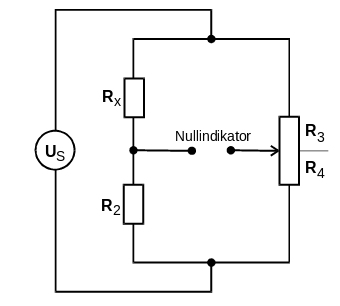
\includegraphics[height=6.25cm]{WheBr.png}
  \caption{Wheatstonesche Brückenschaltung \cite{anleitung}}
  \label{fig:WheBr}
\end{figure}

Der unbekannte Widerstand ist wie man aus der Gleichung
\eqref{eqn:AllgBrW} entnehmen kann

\begin{equation}
  R_x = R_2\frac{R_3}{R_4} = R_2\frac{R_3}{R_G - R_3}
\end{equation}

mit dem Gesamtwiderstand des Potentiometers $R_G$.


\subsection{Messbrücke mit Induktivität und Kapazität}

Bei der Messung von Kapazitäten und Induktivitäten muss beachtet werden, dass
ein komplexer Widerstand, die sogenannte Impedanz, existiert.
Daher muss hier mit einer Wechselstromquelle gearbeitet werden.

\newpage

Für eine ideale Kapazität $C$ ist die Impedanz definiert als

\begin{equation}
  Z_C = - \frac{i}{\omega C} ,
\end{equation}

während sie für eine ideale Induktivität $L$ definiert ist als

\begin{equation}
  Z_L = i \omega L .
\end{equation}

Bei der Brückenschaltung zur Messung dieser komplexen Widerstände sind
die Widerstände $R_x$ und $R_2$ durch Kapazitäten $C_x$ und $C_2$ oder
durch Induktivitäten $L_x$ und $L_2$ ausgetauscht.
Daraus ergibt sich dann über die Kirchhoffschen Gesetze bei einer
genullten Brückenspannung die unbekannte Kapazität

\begin{equation}
  C_x = C_2\frac{R_4}{R_3}
  \label{eqn:KapId}
\end{equation}

von beispielsweise einem Kondensator oder die unbekannte Induktivität

\begin{equation}
  L_x = L_2\frac{R_3}{R_4}
  \label{eqn:IndId}
\end{equation}

von beispielsweise einer Spule.

Wie bereits erwähnt gilt dies nur für ideale Impedanzen, bei realen
Impedanzen muss man zum Beispiel dielektrische Verluste beim Kondensator
oder Wärmeverluste bei einer Spule beachten. Zur Vereinfachung kann man
sich eine reale Impedanz einfach vorstellen als Impedanz mit einem in Reihe
dahinter geschalteten Widerstand wie in Abbildung \ref{fig:ReiheImp}.

\begin{figure}
  \centering
  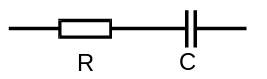
\includegraphics[height=1.5cm]{ReiheImp.png}
  \caption{Ersatzschaltbild eines realen Kondensators \cite{anleitung}}
  \label{fig:ReiheImp}
\end{figure}

Um die Brückenspannung nun auf Null zu setzen muss hinter der zweiten
Kapazität $C_2$ oder der zweiten Induktivität $L_2$ ein weiterer
variabler Widerstand $R_2$ geschaltet werden. In den Abbildungen
\ref{fig:KapBr} und \ref{fig:IndBr} sind die jeweiligen Brückenschaltungen
dargestellt.

\newpage

\begin{figure}[h]
  \centering
  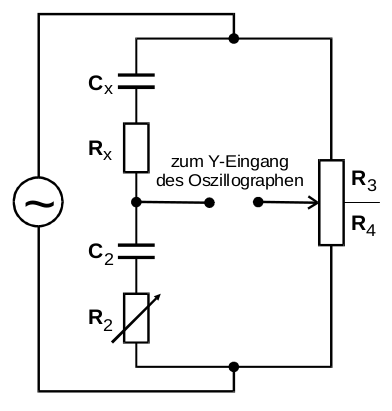
\includegraphics[height=6.25cm]{KapBr.png}
  \caption{Kapazitätsmessbrücke für reale Kondensatoren \cite{anleitung}}
  \label{fig:KapBr}
\end{figure}

\begin{figure}[h]
  \centering
  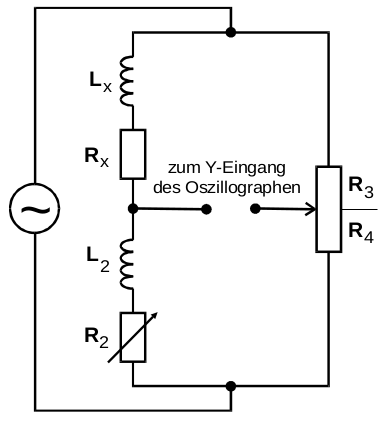
\includegraphics[height=6.25cm]{IndBr.png}
  \caption{Induktivitätsmessbrücke für reale Spulen \cite{anleitung}}
  \label{fig:IndBr}
\end{figure}

Bei den Widerständen für reale Kapazitäten und Induktivitäten muss nun
der unbekannte in Reihe geschaltete Verlustwiderstand $R$ mit einbezogen
werden:

\begin{equation}
  Z_{C_r} = R_C -\frac{i}{\omega C}
\end{equation}

\begin{equation}
  Z_{L_r} = R_L + i \omega L
\end{equation}

Die Kapazität $C_x$ und die Induktivität $L_x$ lassen sich ebenso wie
in den idealen Fällen \eqref{eqn:KapId} und \eqref{eqn:IndId} berechnen.
Die Verlustwiderstände berechnen sich jeweils über die bereits bekannte
Abgleichsbedingung \eqref{eqn:AllgBrW}.


\subsection{Maxwell-Brücke}

Die Maxwellsche Brückenschaltung ist eine weitere Schaltung, mit der man
den Widerstand einer realen Spule bestimmen kann.
Die variablen Widerstände $R_3$ und $R_4$ sind bei dieser Schaltung nicht mehr
in einem Potentiometer vereint, sondern einzeln in die Schaltung eingebaut,
da $R_4$ zusätzlich mit einem annähernd idealen Kondensator
parallel geschaltet wird.
Wo in der einfachen Induktions-Brückenschaltung in Abbildung \ref{fig:IndBr}
eine bekannte reale Spule aus den Elementen $R_2$ und $L_2$ benötigt wurde,
wird hier nur ein fester Widerstand $R_2$ benötigt. Der Aufbau ist in
Abbildung \ref{fig:MaxBr} dargestellt.

\begin{figure}[h]
  \centering
  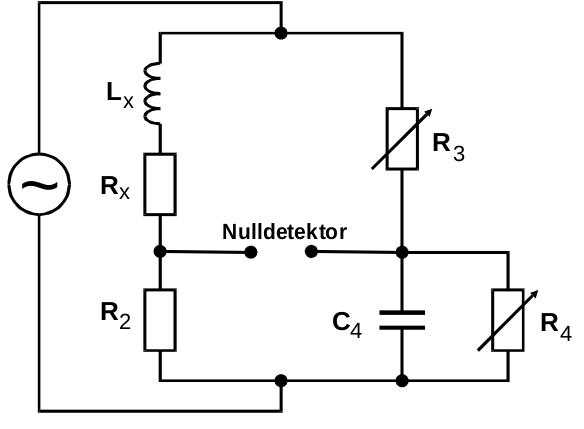
\includegraphics[height=6.25cm]{MaxBr.png}
  \caption{Maxwellsche Brückenschaltung \cite{anleitung}}
  \label{fig:MaxBr}
\end{figure}

Die Impedanz der unbekannten realen Spule beträgt
\begin{equation}
  Z_x = R_x + i\omega L_x
\end{equation}
und die der Kondensator-Parallelschaltung
\begin{equation}
  Z_4 = \frac{R_4 - i\omega C_4R_4^2}{1 + \omega^2 C_4^2R_4^2} .
\end{equation}
Daraus folgt dann über die Kirchhoffschen Gesetze für den Widerstand
\begin{equation}
  R_x = R_2 \frac{R_3}{R_4}
\end{equation}
und für die Induktivität
\begin{equation}
  L_x = R_2 R_3 C_4 .
\end{equation}


\subsection{Wien-Robinson-Brücke}

Bei der Wien-Robinson-Brückenschaltung wird, anders als bei den bisher
vorgestellten Schaltungen, kein unbekannter Widerstand bestimmt.
Stattdessen versucht man hier eine Abhängigkeit zwischen der Brückenspannung
$U_B$ und der Schwingungsfrequenz \omega des Wechselstroms herauszufinden.
Den Aufbau dieser Schaltung kann man in Abbildung \ref{fig:WRBr} erkennen.

\begin{figure}[h]
  \centering
  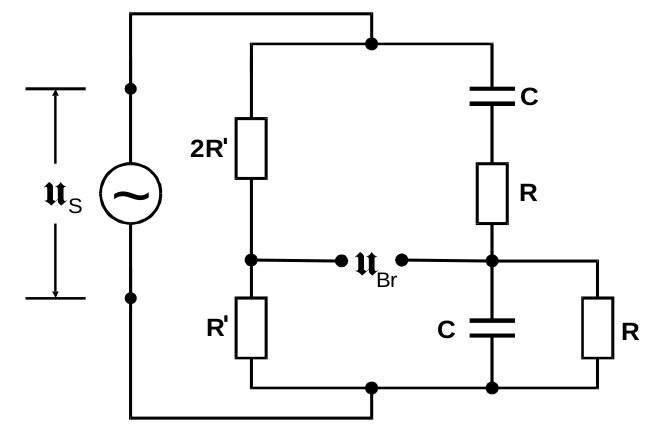
\includegraphics[height=6.25cm]{WRBr.png}
  \caption{Wien-Robinson-Brückenschaltung \cite{anleitung}}
  \label{fig:WRBr}
\end{figure}

Aus der allgemeinen Gleichung für die Brückenspannung \eqref{eqn:Brs}
folgt dann für den Betrag des Verhätnisses zwischen Brücken- und Speisespannung
\begin{equation}
  \Bigl|\frac{U_B}{U_S}\Bigr|^2 = \frac{(\omega^2 R^2 C^2 -1)^2}{9\Bigl
  ((1-\omega^2 R^2 C^2)^2 + 9 \omega^2 R^2 C^2\Bigr)} .
  \label{eqn:WRBG}
\end{equation}
Die Brückenspannung wird dann also bei Kreisfrequenz
\begin{equation}
  \omega = \omega_0 = \frac{1}{RC}
\end{equation}
Null.
Nun wird das Frequenzverhältnis
\begin{equation}
  \Omega = \frac{\omega}{\omega_0}
\end{equation}
eingeführt, sodass die Gleichung \eqref{eqn:WRBG} durch
\begin{equation}
    \Bigl|\frac{U_B}{U_S}\Bigr|^2 = \frac{1}{9} \frac{(\Omega^2-1)^2}
    {(1-\Omega^2)^2 + 9\Omega^2}
    \label{eqn:wienrobin1/9}
\end{equation}
dargestellt werden kann.
An diesen Ergebnissen erkennt man, dass die Wien-Robinson-Brücke wie ein
Filter fungiert, der in dem kontinuierlichen Frequenzspektrum ein Minumum
an der Frequenz $\omega_0$ anzeigt. Dadurch ist es möglich mit dieser
Brückenschaltung den sogenannten Klirrfaktor einer Wechselstromquelle zu
bestimmen. Dieser Faktor gibt sozusagen die Qualität des Gerätes an, da er das
Verhältnis zwischen den Grundwellen und den unerwünschten Oberwellen angibt.
Denn auch bei der Frequenz $\omega_0$ ist die gemessene Brückenspannung nicht
Null. Man misst noch eine geringe Spannung, die durch die Oberwellen erzeugt
wird. Der Klirrfaktor ist definiert durch die Gleichung
\begin{equation}
  k = \frac{\sqrt{\sum_{n=2}^N U_n^2}}{U_1}
  \label{eqn:klirrf}
\end{equation}
mit der Amplitude $U_1$ der Grundwelle und $U_2$ bis $U_N$ der Oberwellen.
